% !TeX root = ../main.tex
\section{Arquitectura base con el modelo C4}
\label{sec:clab-c4}

El nivel 1 delimita CLAB respecto de las personas y de los sistemas externos;
el nivel 2 lo descompone en aplicaciones y almacenes. En C4, un contenedor no
significa necesariamente un contenedor Docker: también puede ser una SPA, un
servicio o una base de datos\cite{clabC4Contenedores}. Los archivos editables
están en \texttt{docs/diagramas/}; sus figuras vectoriales están en
\texttt{docs/figuras/}.

\subsection{Contexto: nivel 1}

El docente consulta horarios, reserva y reporta fallas; el coordinador planifica
el uso académico; el administrador de laboratorio mantiene recursos y registra
asistencia; el administrador del sistema gestiona accesos y bloqueos. El SGA
se muestra como sistema externo de integración futura, sin conexión activa ni
API acordada; no es una dependencia para ejecutar E1 ni un compromiso de
integración durante el periodo.

\begin{figure*}[!t]
  \centering
  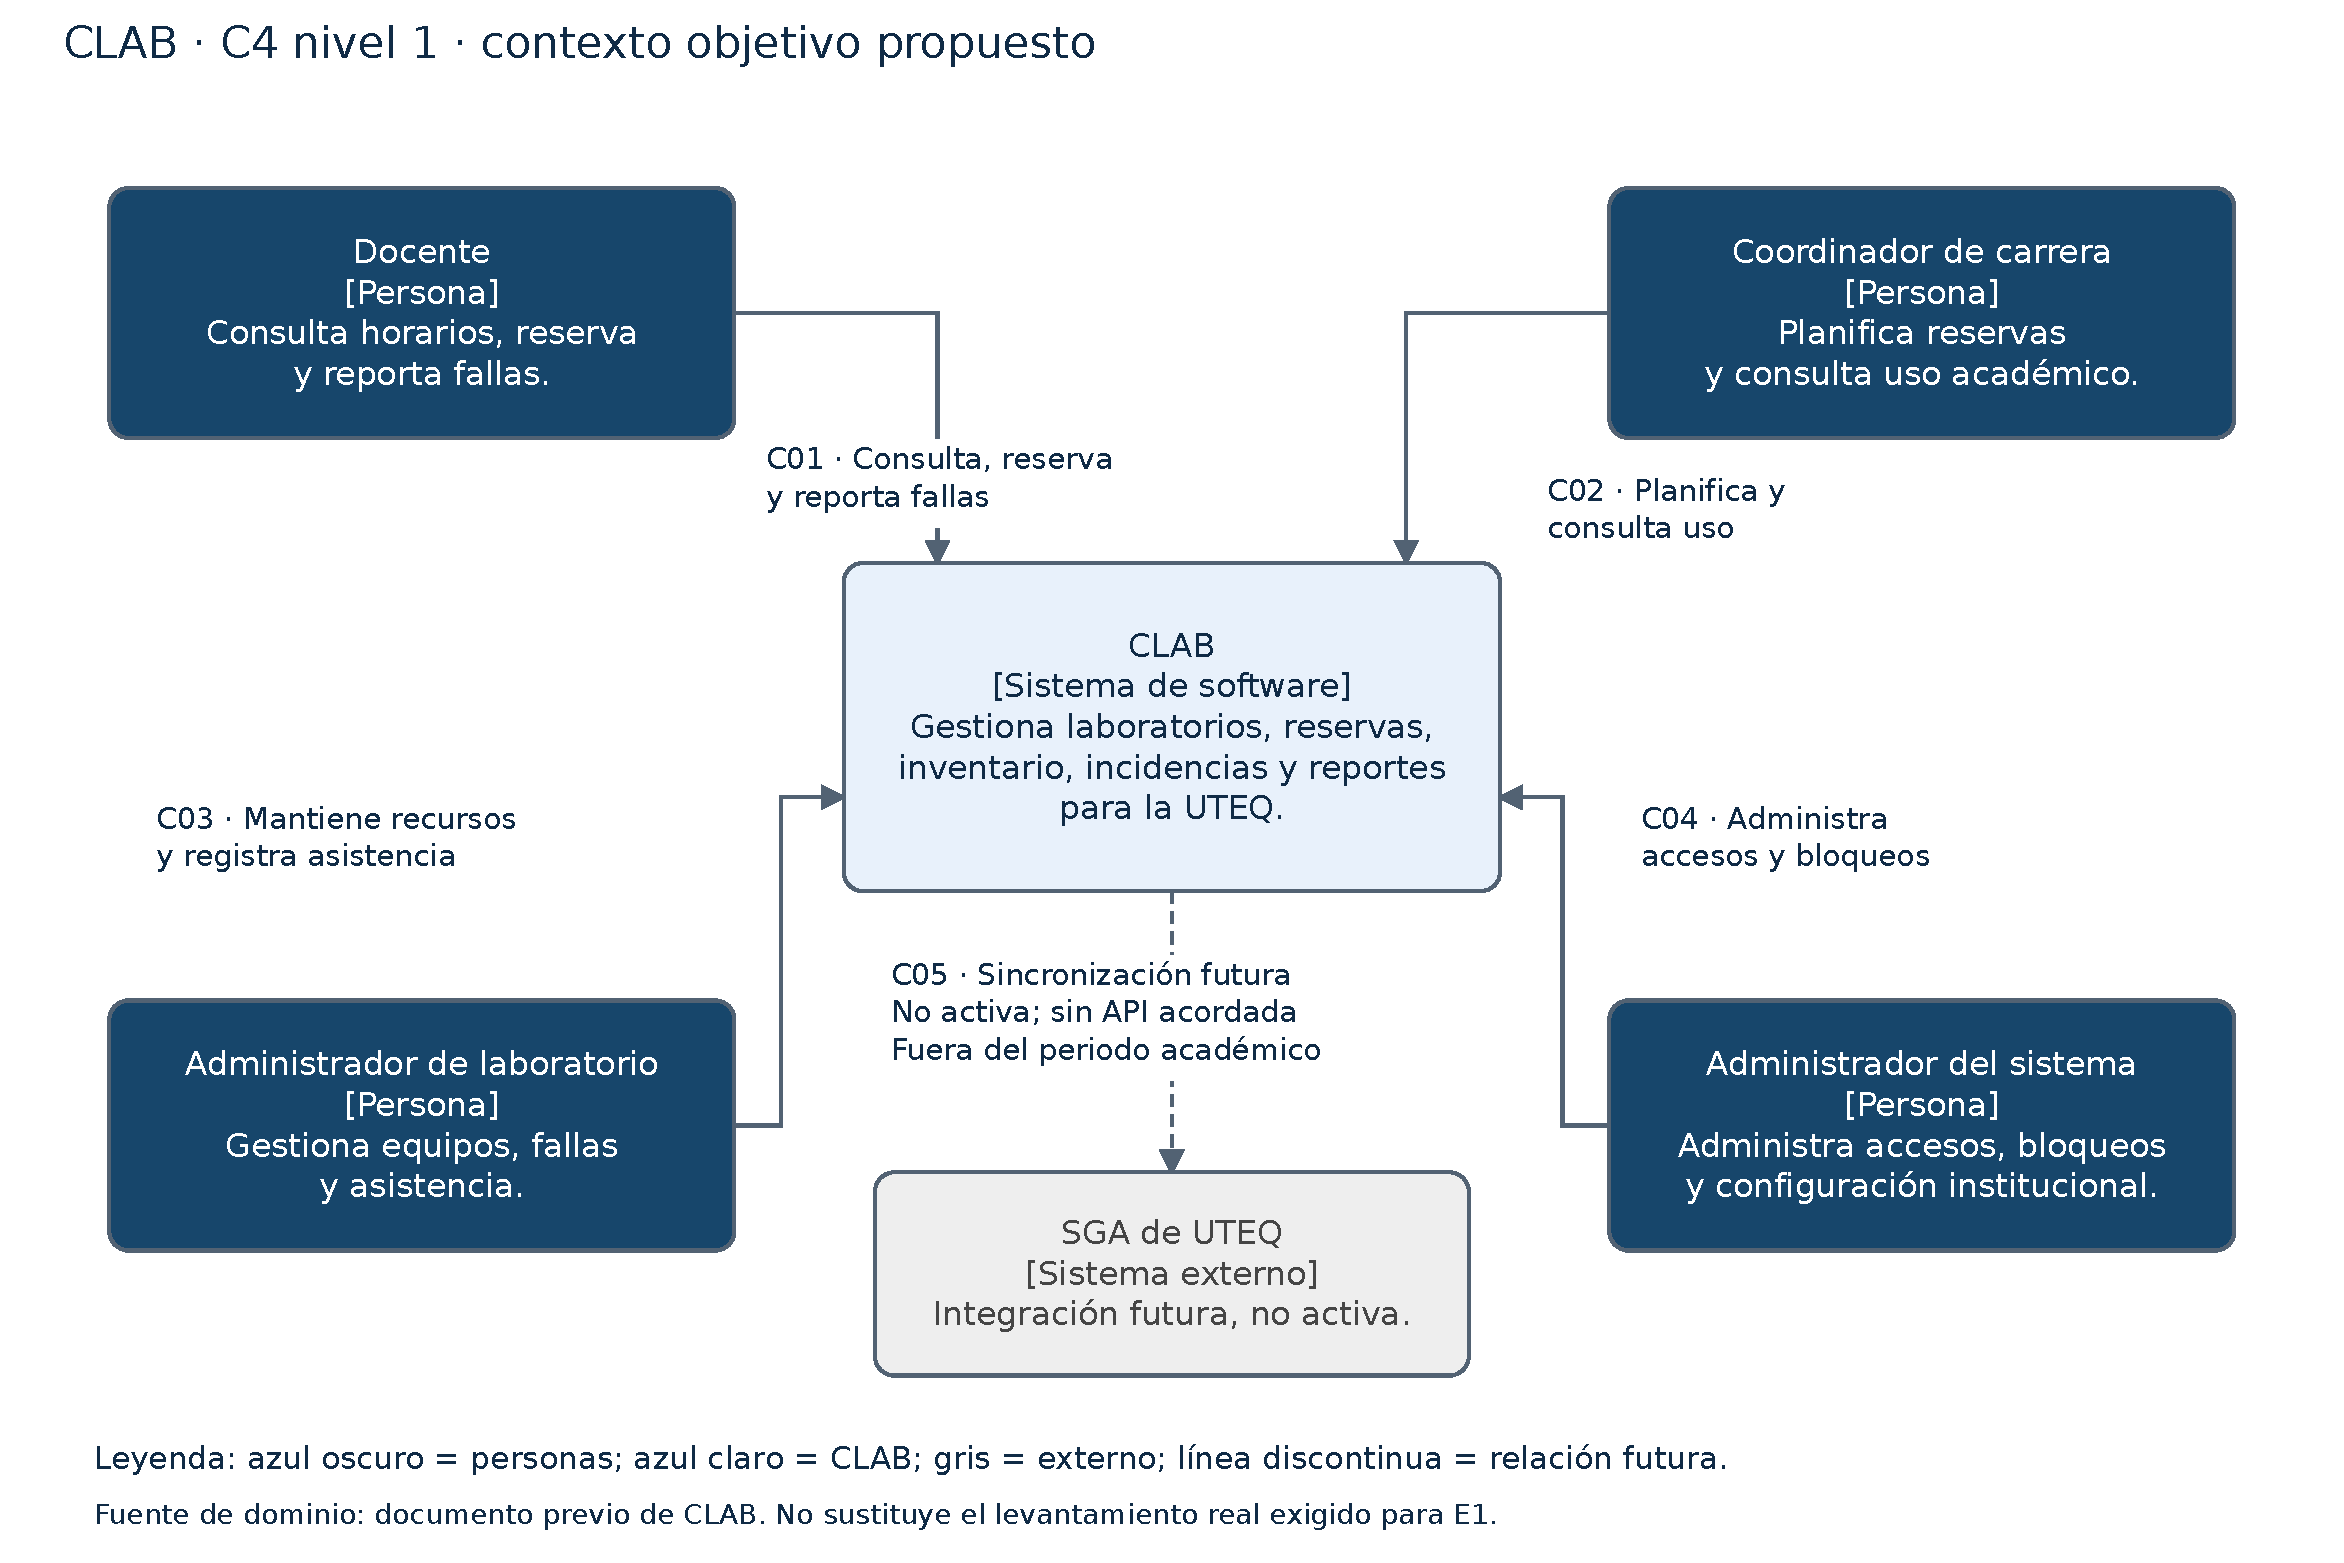
\includegraphics[width=\textwidth,height=0.40\textheight,keepaspectratio]{figuras/c4-contexto.pdf}
  \caption{Contexto objetivo de CLAB. La relación discontinua con el SGA es
  futura, no implementada.}
  \label{fig:clab-contexto}
\end{figure*}

\subsection{Contenedores: nivel 2}

La arquitectura objetivo agrupa los doce módulos del legado en cuatro servicios
con almacenamiento exclusivo, de acuerdo con ADR-001. La SPA no escribe en
bases de datos. No hay consultas SQL entre almacenes ni un broker propuesto
como si estuviera instalado. La auditoría y los cambios se registran localmente
en la transacción de origen, y la vista central los incorpora posteriormente.
La agrupación y los flujos son una propuesta pendiente de aceptación del equipo;
no acreditan que los módulos del backend legado ya se hayan migrado.

\begin{figure*}[!t]
  \centering
  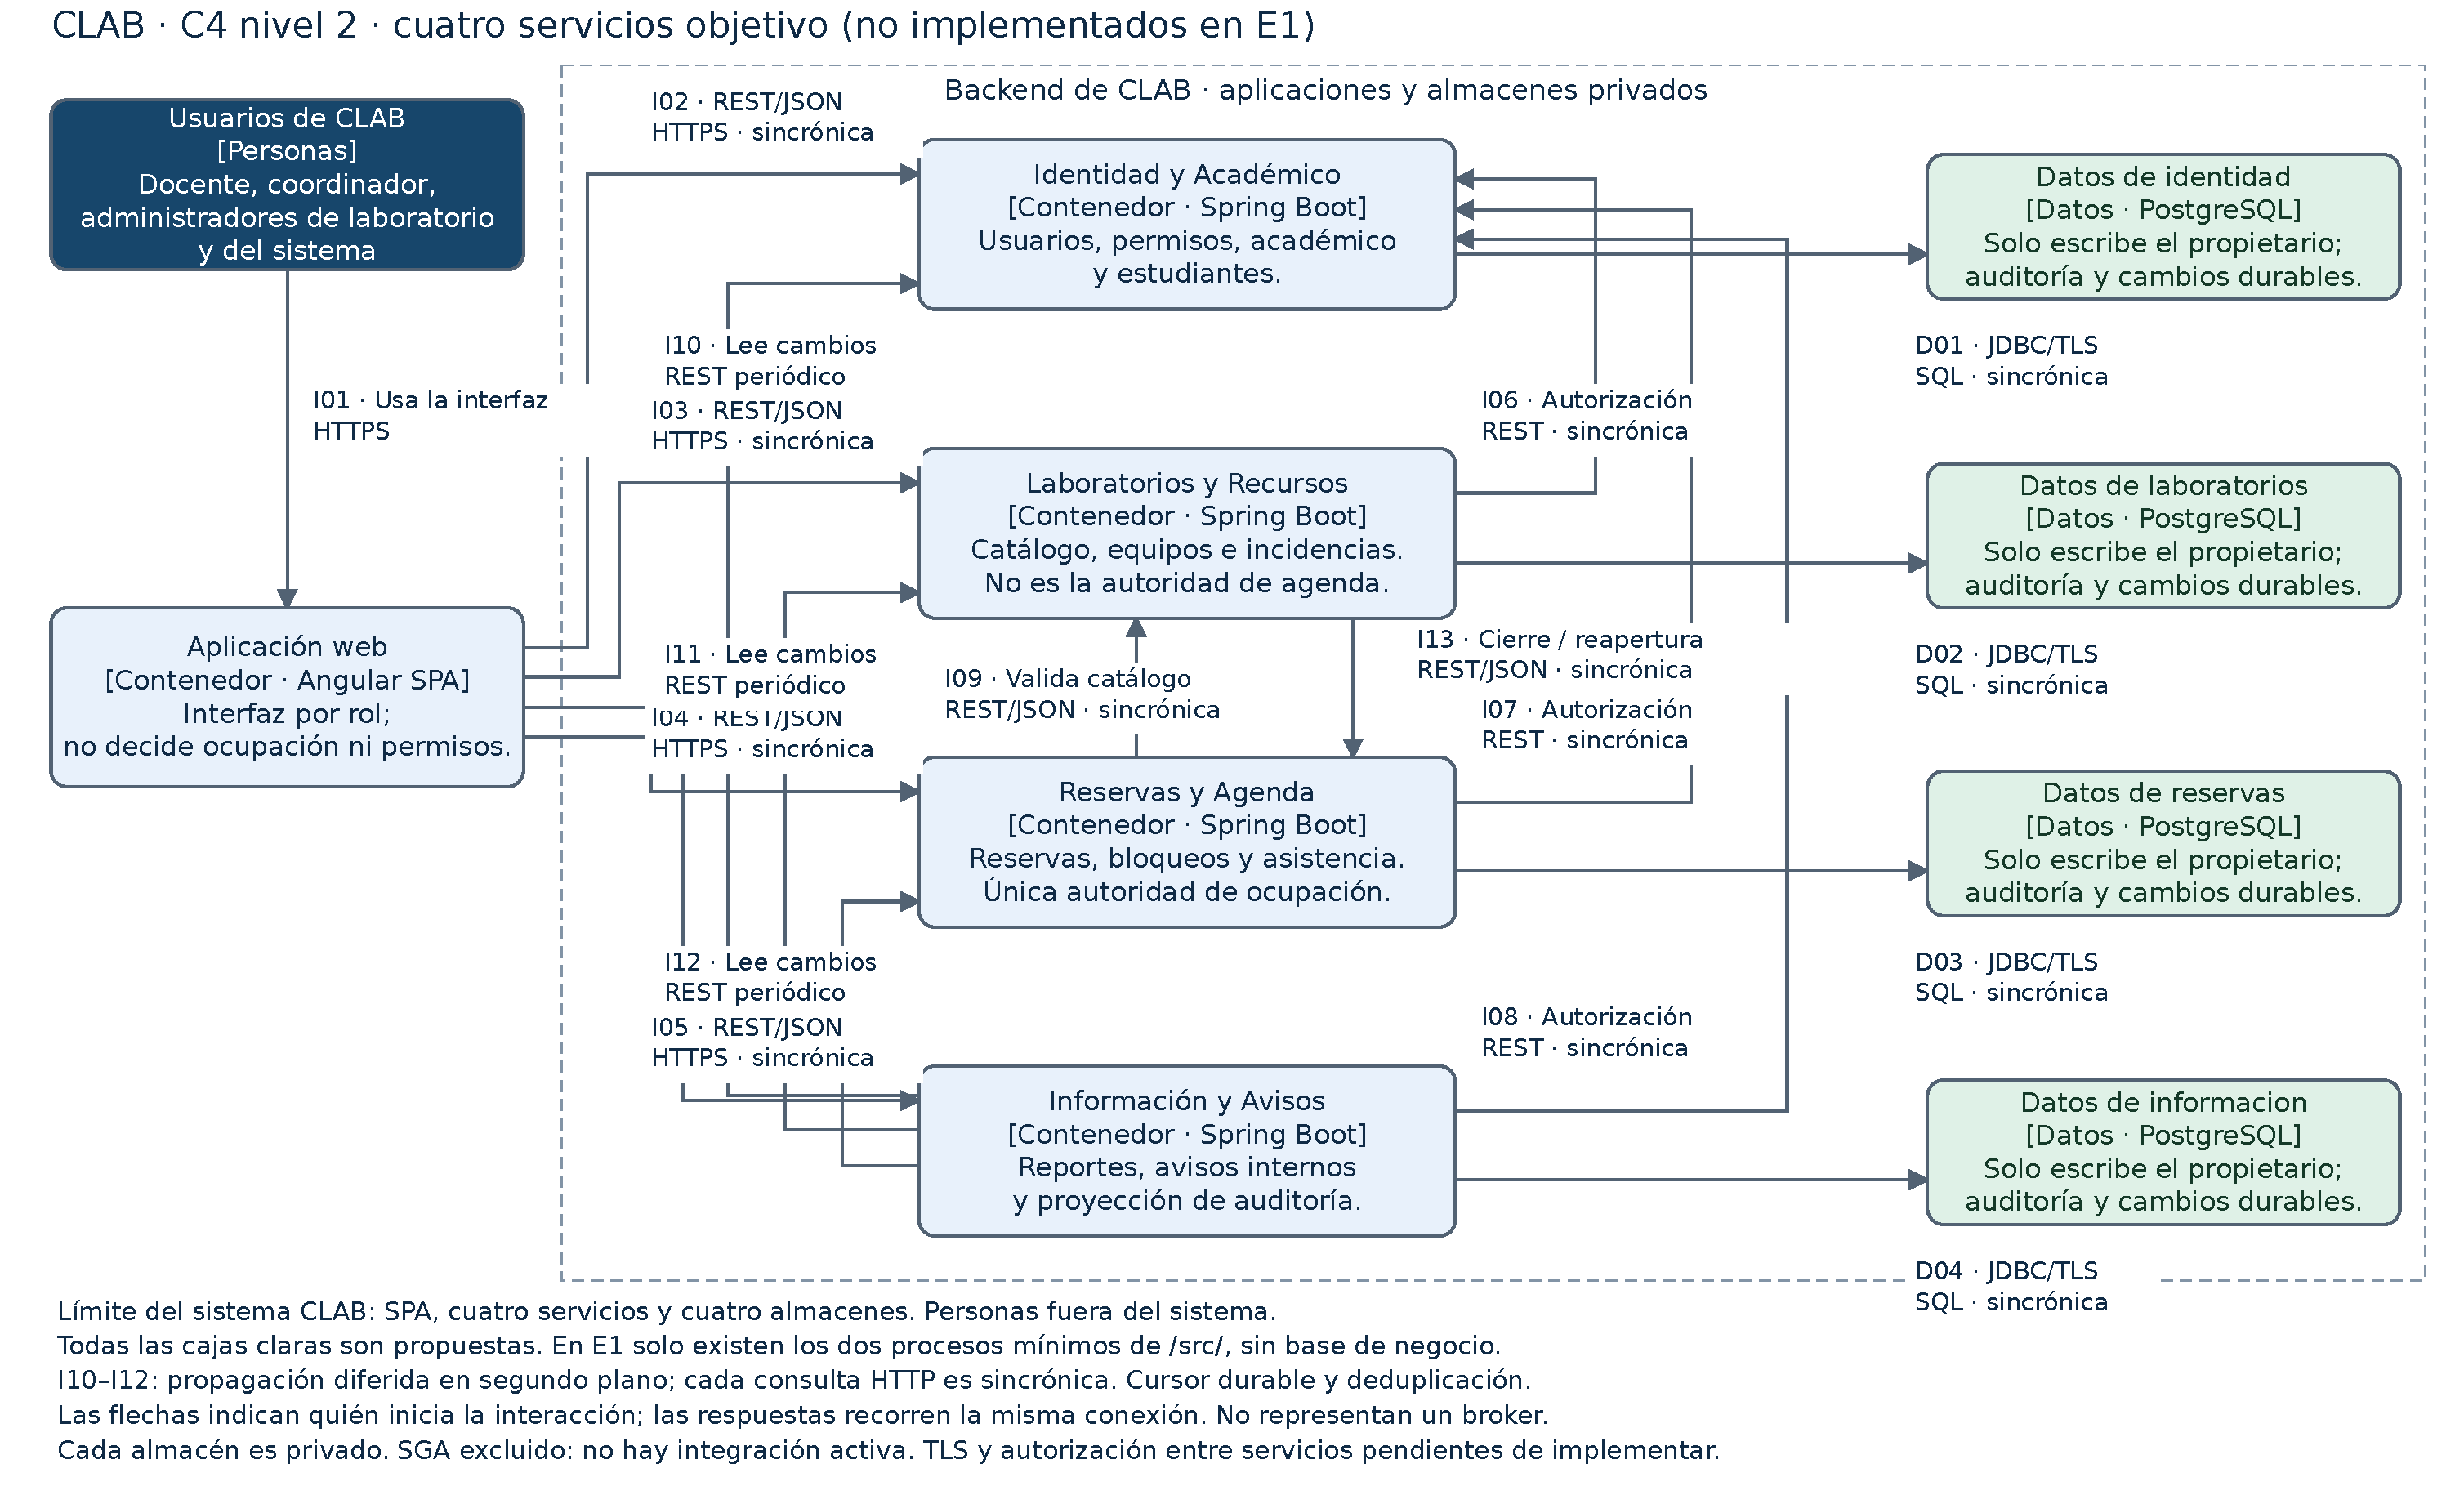
\includegraphics[width=\textwidth,height=0.48\textheight,keepaspectratio]{figuras/c4-contenedores.pdf}
  \caption{Contenedores objetivo de CLAB. Los identificadores permiten
  rastrear las interacciones; no representan funcionalidad implementada en E1.}
  \label{fig:clab-contenedores}
\end{figure*}

\subsection{Lectura y límites de las interacciones}

Las flechas indican el iniciador; la respuesta vuelve por la misma conexión.
Los identificadores son un inventario de interfaces de arquitectura para
contrastarlo con el modelo de comunicación y ADR-002, no una sustitución de
esos entregables.

\begin{description}
  \item[I01:] personas a SPA por HTTPS.
  \item[I02--I05:] SPA a Identidad, Laboratorios, Reservas e Información,
  respectivamente, mediante REST/JSON sincrónico sobre HTTPS. Cada servicio
  aplica permisos; ocultar un botón en Angular no es autorización.
  \item[I06--I08:] Laboratorios, Reservas e Información consultan Identidad
  mediante REST sincrónico para autorizar peticiones protegidas. Si Identidad
  no responde, no se autoriza la operación; esto introduce un punto común de
  dependencia que deberá medirse.
  \item[I09:] Reservas valida el catálogo de Laboratorios mediante REST/JSON
  sincrónico antes de confirmar una nueva reserva. La ocupación se decide en
  Reservas, no con una copia del calendario en Laboratorios.
  \item[I10--I12:] Información consulta los cambios de Identidad, Laboratorios
  y Reservas, respectivamente, mediante REST periódico. La incorporación a
  reportes y avisos es diferida: cada HTTP espera respuesta, pero la transacción
  original no espera que la proyección se actualice. Cursores, retención,
  autenticación de máquina y reintentos todavía requieren implementación.
  El contrato de cambios debe limitarse a los datos necesarios para cada
  proyección: no debe exponer contraseñas, hashes, tokens ni secretos de sesión.
  \item[I13:] Laboratorios solicita a Reservas el cierre o la reapertura de
  la barrera operativa mediante REST/JSON sincrónico, con identificador estable
  y revisión. Reservas autoriza y persiste el cambio sin volver a llamar a
  Laboratorios desde este manejador. Ante un resultado desconocido se consulta
  o reintenta la misma solicitud; no se infiere que haya fallado por un timeout.
  \item[D01--D04:] cada servicio accede únicamente a su propio almacén mediante
  JDBC y SQL, con TLS previsto para conexiones de red. Persistencia y registros
  de cambios durables no están presentes en los dos servicios mínimos de E1.
\end{description}

No se propone invocar servicios de negocio desde Información para ejecutar
escrituras. Si Información está detenido, la agenda debe poder confirmar y
mantener sus registros locales. Si Laboratorios o Identidad están inaccesibles,
una nueva reserva que dependa de ellos no se confirma. Esto es aislamiento
parcial por operación, no disponibilidad total frente a cualquier fallo.

Para RF-P04, Laboratorios solo publica fuera de servicio después de confirmar
la barrera en Reservas; en caso contrario muestra cierre pendiente. La barrera
se verifica bajo el mismo bloqueo por laboratorio que cada confirmación de
reserva. Las reservas previas se conservan, sin cancelación automática ni
autorización de uso físico del espacio cerrado. Para reabrir, el catálogo pasa
primero a apertura pendiente, después Reservas retira únicamente su barrera
operativa y finalmente el catálogo publica activo. Un fallo no debe provocar
que se anuncie un cierre sin barrera o una reapertura sin confirmación.
Los estados, revisiones y reintentos de este diseño se detallan en ADR-001.

\subsection{Correspondencia con el esqueleto de E1}

En el código revisado existen \path{servicio-reservas} y
\path{servicio-laboratorios}. La petición
\path{/api/reservas/comunicacion} consulta
\path{/api/laboratorios/info} por HTTP y devuelve el mensaje recibido.
Esa relación es el antecedente técnico de I09, pero todavía no valida un
laboratorio real ni crea reservas. Los procesos se enlazan a la interfaz local;
HTTPS, autorización, bases privadas y propagación de cambios son diseño futuro.
No se ha ejecutado ni validado la arquitectura completa de cuatro servicios.

\paragraph{Evidencia de diseño y asistencia.}
Estos diagramas digitales no sustituyen el primer bosquejo ni las dos
fotografías reales de sesiones del equipo. Se prepararon con asistencia de
IA (OpenAI, GPT-6.1 Sol); no acreditan participación presencial ni sesiones
que no estén documentadas por los integrantes.
